% Practice Test 04 — Texas Edition
% Questions: 30 (21 MC + 9 SA)
% Generated by scripts/generate_practice_tests.py

\begin{practiceQuestion}{1-3-q06}{mc}
\begin{questionText}
On a proportional graph, the point $(1, r)$ represents:
\end{questionText}
\choiceA{The $x$-intercept}
\choiceB{The constant of proportionality}
\choiceC{The slope of the line}
\choiceD{Both B and C}
\correctAnswer{D}
\explanation{At $x = 1$, $y = k \times 1 = k$. So the point $(1, r)$ gives the constant of proportionality, which is also the slope.}
\end{practiceQuestion}

\begin{practiceQuestion}{1-6-q06}{mc}
\begin{questionText}
Small paint can: $\frac{3}{4}$ gallon for $\$18$. Large can: $1\frac{1}{2}$ gallons for $\$33$. Which is the better buy?
\end{questionText}
\choiceA{Small, at $\$22$/gal}
\choiceB{Large, at $\$22$/gal}
\choiceC{Small, at $\$24$/gal}
\choiceD{Large, at $\$24$/gal}
\correctAnswer{B}
\explanation{Small: $18 \div 0.75 = \$24$/gal. Large: $33 \div 1.5 = \$22$/gal. The large can is $\$2$/gal cheaper.}
\end{practiceQuestion}

\begin{practiceQuestion}{2-1-q04}{mc}
\begin{questionText}
A class has $32$ students. If $75\%$ passed the test, how many students passed?
\end{questionText}
\choiceA{$20$}
\choiceB{$24$}
\choiceC{$25$}
\choiceD{$28$}
\correctAnswer{B}
\explanation{$75\% = 0.75$. Multiply: $0.75 \times 32 = 24$ students passed.}
\end{practiceQuestion}

\begin{practiceQuestion}{2-3-q11}{mc}
\begin{questionText}
Miranda says that a $50\%$ increase followed by a $50\%$ decrease gives back the original price. Is she correct?
\end{questionText}
\choiceA{Yes, because the two changes cancel out}
\choiceB{No, the result is less than the original}
\choiceC{No, the result is more than the original}
\choiceD{It depends on the starting price}
\correctAnswer{B}
\explanation{Start with $\$100$. Increase $50\%$: $\$150$. Decrease $50\%$: $150 \times 0.50 = \$75$. That is less than $\$100$.}
\end{practiceQuestion}

\begin{practiceQuestion}{2-6-q13}{mc}
\begin{questionText}
You want to earn $\$200$ in interest in $4$ years at $5\%$ simple interest. How much must you deposit?
\end{questionText}
\choiceA{$\$800$}
\choiceB{$\$1{,}000$}
\choiceC{$\$1{,}200$}
\choiceD{$\$2{,}000$}
\correctAnswer{B}
\explanation{$200 = P \times 0.05 \times 4$ → $200 = 0.20P$ → $P = \$1{,}000$.}
\end{practiceQuestion}

\begin{practiceQuestion}{2-8-q24}{sa}
\begin{questionText}
Bank A pays $3\%$ interest per year. Bank B pays $1\%$ per year. You deposit $\$1{,}000$ in each for $1$ year. How much more interest does Bank A earn?
\end{questionText}
\correctAnswer{$\$20$}
\explanation{Bank A: $1{,}000 \times 0.03 = \$30$. Bank B: $1{,}000 \times 0.01 = \$10$. Difference: $30 - 10 = \$20$.}
\end{practiceQuestion}

\begin{practiceQuestion}{2-9-q28}{gmc}
\begin{questionText}
The line graph shows a student's savings account balance over $4$ months. Between which two months did the balance increase the most?

\begin{center}
\begin{tikzpicture}[scale=0.8]
  \draw[thick,->] (0,0) -- (5.5,0) node[right] {Month};
  \draw[thick,->] (0,0) -- (0,5) node[above] {\$};
  \foreach \x/\label in {1/Jan, 2/Feb, 3/Mar, 4/Apr} {
    \draw (\x,-0.1) -- (\x,0.1);
    \node[below] at (\x,-0.15) {\footnotesize \label};
  }
  \foreach \y/\label in {1/100, 2/200, 3/300, 4/400} {
    \draw (-0.1,\y) -- (0.1,\y);
    \node[left] at (-0.15,\y) {\footnotesize \$\label};
  }
  \draw[thick,funBlue,mark=*] plot coordinates {(1,1) (2,1.5) (3,3) (4,3.5)};
  \node[above] at (1,1) {\footnotesize \$100};
  \node[above] at (2,1.5) {\footnotesize \$150};
  \node[above] at (3,3) {\footnotesize \$300};
  \node[above right] at (4,3.5) {\footnotesize \$350};
\end{tikzpicture}
\end{center}
\end{questionText}
\choiceA{Jan to Feb}
\choiceB{Feb to Mar}
\choiceC{Mar to Apr}
\choiceD{Jan to Mar}
\correctAnswer{B}
\explanation{Jan to Feb: $\$50$ increase. Feb to Mar: $\$150$ increase. Mar to Apr: $\$50$ increase. The biggest increase is Feb to Mar.}
\end{practiceQuestion}

\begin{practiceQuestion}{2-10-q25}{sa}
\begin{questionText}
Explain in your own words why compound interest grows faster than simple interest.
\end{questionText}
\correctAnswer{You earn interest on your previously earned interest}
\explanation{Each year, the interest earned is added to the principal. The next year, you earn interest on a larger amount, so it grows faster.}
\end{practiceQuestion}

\begin{practiceQuestion}{4-1-q02}{mc}
\begin{questionText}
What is the value of $3x - 5$ when $x = 4$?
\end{questionText}
\choiceA{$2$}
\choiceB{$7$}
\choiceC{$17$}
\choiceD{$-2$}
\correctAnswer{B}
\explanation{Substitute: $3(4) - 5 = 12 - 5 = 7$.}
\end{practiceQuestion}

\begin{practiceQuestion}{4-2-q27}{gmc}
\begin{questionText}
The lengths of the four sides of a quadrilateral are shown below. What is the simplified perimeter?

\begin{center}
\begin{tikzpicture}[scale=0.9]
  \draw[thick, fill=funBlue!10] (0,0) -- (4,0) -- (5,3) -- (1,3) -- cycle;
  \node[below] at (2,0) {$3x + 2$};
  \node[right] at (4.7,1.5) {$x + 1$};
  \node[above] at (3,3) {$2x - 3$};
  \node[left] at (0.3,1.5) {$x + 4$};
\end{tikzpicture}
\end{center}
\end{questionText}
\choiceA{$7x + 4$}
\choiceB{$6x + 4$}
\choiceC{$7x - 4$}
\choiceD{$6x + 10$}
\correctAnswer{A}
\explanation{Add all sides: $(3x + 2) + (x + 1) + (2x - 3) + (x + 4)$. Combine variable terms: $3x + x + 2x + x = 7x$. Combine constants: $2 + 1 - 3 + 4 = 4$. Perimeter: $7x + 4$.}
\end{practiceQuestion}

\begin{practiceQuestion}{5-3-q05}{mc}
\begin{questionText}
Solve $6(x - 1) = -18$.
\end{questionText}
\choiceA{$x = -2$}
\choiceB{$x = 2$}
\choiceC{$x = -4$}
\choiceD{$x = 4$}
\correctAnswer{A}
\explanation{Divide by $6$: $x - 1 = -3$. Add $1$: $x = -2$. Check: $6(-2 - 1) = 6(-3) = -18$ \checkmark.}
\end{practiceQuestion}

\begin{practiceQuestion}{5-4-q29}{gsa}
\begin{questionText}
The bar graph shows how much three students earned. Together they earned a total of $\$31.50$. Student C earned $\dfrac{1}{2}$ as much as Student A. Find how much Student C earned.

\begin{center}
\begin{tikzpicture}[scale=0.5]
  \draw[thick,->] (0,0) -- (0,11) node[above] {Dollars (\$)};
  \draw[thick,->] (0,0) -- (10,0);
  % Bars
  \draw[thick,fill=funBlue!40] (1,0) rectangle (3,8);
  \node[below] at (2,-0.3) {A};
  \node at (2,8.5) {$\$12$};
  \draw[thick,fill=funOrange!40] (4,0) rectangle (6,0);
  \node[below] at (5,-0.3) {B};
  \node at (5,1) {?};
  \draw[thick,fill=funGreen!40] (7,0) rectangle (9,0);
  \node[below] at (8,-0.3) {C};
  \node at (8,1) {?};
  % Y-axis labels
  \foreach \y in {0,2,...,10} {
    \draw (-0.2,\y) -- (0,\y);
    \node[left] at (-0.3,\y) {$\y$};
  }
\end{tikzpicture}
\end{center}

Student A earned $\$12$, and Student C earned $\dfrac{1}{2}$ of Student A's earnings.
\end{questionText}
\correctAnswer{$\$6$}
\explanation{Student C $= \frac{1}{2} \times 12 = \$6$. Check: Student B $= 31.50 - 12 - 6 = \$13.50$. Total: $12 + 13.50 + 6 = 31.50$ \checkmark.}
\end{practiceQuestion}

\begin{practiceQuestion}{5-5-q26}{gmc}
\begin{questionText}
Which inequality is represented by the number line below?

\begin{center}
\begin{tikzpicture}[scale=0.7]
  \draw[thick,->] (-1,0) -- (10,0);
  \foreach \x in {0,...,9} \draw (\x,0.15) -- (\x,-0.15) node[below] {$\x$};
  \draw[thick,funBlue,->] (5,0) -- (10,0);
  \draw[thick,funBlue,fill=white] (5,0) circle (4pt);
\end{tikzpicture}
\end{center}
\end{questionText}
\choiceA{$x \geq 5$}
\choiceB{$x > 5$}
\choiceC{$x \leq 5$}
\choiceD{$x < 5$}
\correctAnswer{B}
\explanation{An open circle at $5$ with shading to the right means $x > 5$ (not including $5$).}
\end{practiceQuestion}

\begin{practiceQuestion}{5-6-q13}{mc}
\begin{questionText}
True or false: The graph of $x < 5$ and $x \leq 5$ look exactly the same.
\end{questionText}
\choiceA{True — both shade to the left of $5$}
\choiceB{False — $x < 5$ has an open circle, $x \leq 5$ has a closed circle}
\choiceC{False — they shade in different directions}
\choiceD{True — the circle type does not matter}
\correctAnswer{B}
\explanation{$x < 5$ uses an open circle (not including $5$) while $x \leq 5$ uses a closed circle (including $5$). Both shade left.}
\end{practiceQuestion}

\begin{practiceQuestion}{6-2-q13}{mc}
\begin{questionText}
A drawing uses $1$ cm $= 6$ m. It is redrawn at $1$ cm $= 2$ m. The original drawing is $8$ cm by $5$ cm. What is the perimeter of the new drawing?
\end{questionText}
\choiceA{$26$ cm}
\choiceB{$39$ cm}
\choiceC{$78$ cm}
\choiceD{$120$ cm}
\correctAnswer{C}
\explanation{Scale ratio: $\frac{6}{2} = 3$. New dimensions: $8 \times 3 = 24$ cm and $5 \times 3 = 15$ cm. New perimeter: $2(24 + 15) = 78$ cm.}
\end{practiceQuestion}

\begin{practiceQuestion}{6-3-q15}{mc}
\begin{questionText}
Which condition makes it impossible to draw a triangle?
\end{questionText}
\choiceA{Sides $5$, $12$, $13$}
\choiceB{Sides $7$, $7$, $7$}
\choiceC{Sides $1$, $1$, $3$}
\choiceD{Sides $8$, $15$, $17$}
\correctAnswer{C}
\explanation{$1 + 1 = 2 < 3$. The triangle inequality fails. The other three sets all satisfy the triangle inequality.}
\end{practiceQuestion}

\begin{practiceQuestion}{6-4-q19}{sa}
\begin{questionText}
Two angles of a triangle are $72°$ and $53°$. What is the third angle?
\end{questionText}
\correctAnswer{$55°$}
\explanation{$180° - 72° - 53° = 55°$.}
\end{practiceQuestion}

\begin{practiceQuestion}{6-5-q27}{gmc}
\begin{questionText}
The diagram shows a cone being sliced. Which cut produces a circular cross-section?

\begin{center}
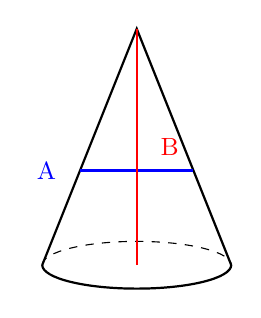
\begin{tikzpicture}[scale=0.6]
  % Cone
  \draw[thick] (-2,0) -- (0,5) -- (2,0);
  \draw[thick] (-2,0) arc[start angle=180,end angle=360,x radius=2,y radius=0.5];
  \draw[dashed] (-2,0) arc[start angle=180,end angle=0,x radius=2,y radius=0.5];
  % Cut A - horizontal
  \draw[thick,blue] (-1.2,2) -- (1.2,2);
  \node[left,blue] at (-1.5,2) {\small A};
  % Cut B - vertical through apex
  \draw[thick,red] (0,0) -- (0,5);
  \node[right,red] at (0.3,2.5) {\small B};
\end{tikzpicture}
\end{center}
\end{questionText}
\choiceA{Cut A (horizontal)}
\choiceB{Cut B (vertical through apex)}
\choiceC{Both cuts}
\choiceD{Neither cut}
\correctAnswer{A}
\explanation{Cut A (horizontal, parallel to the base) produces a circle. Cut B (vertical through the apex) produces a triangle.}
\end{practiceQuestion}

\begin{practiceQuestion}{6-8-q24}{sa}
\begin{questionText}
Two similar triangles have corresponding sides $6$ and $10$. If the perimeter of the smaller triangle is $18$ cm, what is the perimeter of the larger triangle?
\end{questionText}
\correctAnswer{$30$ cm}
\explanation{Scale factor: $\frac{10}{6} = \frac{5}{3}$. Larger perimeter: $18 \times \frac{5}{3} = 30$ cm.}
\end{practiceQuestion}

\begin{practiceQuestion}{7-4-q01}{mc}
\begin{questionText}
A composite shape is made of a rectangle that is $10$ cm by $4$ cm and a triangle with base $10$ cm and height $3$ cm attached to one side. What is the total area?
\end{questionText}
\choiceA{$40$ cm$^2$}
\choiceB{$55$ cm$^2$}
\choiceC{$70$ cm$^2$}
\choiceD{$120$ cm$^2$}
\correctAnswer{B}
\explanation{Rectangle: $10 \times 4 = 40$ cm$^2$. Triangle: $\frac{1}{2} \times 10 \times 3 = 15$ cm$^2$. Total: $40 + 15 = 55$ cm$^2$.}
\end{practiceQuestion}

\begin{practiceQuestion}{7-5-q02}{mc}
\begin{questionText}
What is the surface area of a rectangular prism with length $5$ cm, width $3$ cm, and height $2$ cm?
\end{questionText}
\choiceA{$30$ cm$^2$}
\choiceB{$62$ cm$^2$}
\choiceC{$46$ cm$^2$}
\choiceD{$31$ cm$^2$}
\correctAnswer{B}
\explanation{$SA = 2(5 \times 3) + 2(5 \times 2) + 2(3 \times 2) = 30 + 20 + 12 = 62$ cm$^2$.}
\end{practiceQuestion}

\begin{practiceQuestion}{7-6-q15}{mc}
\begin{questionText}
A sandbox is $6$ ft long, $4$ ft wide, and $1$ ft deep. Sand costs \$$2$ per cubic foot. How much does it cost to fill the sandbox?
\end{questionText}
\choiceA{$\$12$}
\choiceB{$\$24$}
\choiceC{$\$48$}
\choiceD{$\$96$}
\correctAnswer{C}
\explanation{$V = 6 \times 4 \times 1 = 24$ ft$^3$. Cost: $24 \times 2 = \$48$.}
\end{practiceQuestion}

\begin{practiceQuestion}{8-1-q21}{sa}
\begin{questionText}
A random sample of $50$ apples from an orchard found that $6$ were bruised. If the orchard has $3{,}000$ apples, about how many are bruised?
\end{questionText}
\correctAnswer{$360$}
\explanation{$\frac{6}{50} = 12\%$. Then $12\%$ of $3{,}000 = 360$.}
\end{practiceQuestion}

\begin{practiceQuestion}{8-2-q03}{mc}
\begin{questionText}
Why do different random samples from the same population often produce different results?
\end{questionText}
\choiceA{Because the population changes each time}
\choiceB{Because of random variation in sample selection}
\choiceC{Because the data is incorrect}
\choiceD{Because the samples are biased}
\correctAnswer{B}
\explanation{Different samples include different individuals, causing natural variation in results.}
\end{practiceQuestion}

\begin{practiceQuestion}{8-4-q21}{sa}
\begin{questionText}
Data: $5, 5, 10, 10, 10, 15, 15$. The mean is $10$. Find the MAD.
\end{questionText}
\correctAnswer{$\approx 3.57$}
\explanation{Deviations: $5+5+0+0+0+5+5 = 20$. MAD $= \frac{20}{7} \approx 2.86$. Wait — let me recalculate: $|5-10|+|5-10|+|10-10|+|10-10|+|10-10|+|15-10|+|15-10| = 5+5+0+0+0+5+5 = 20$. MAD $= \frac{20}{7} \approx 2.86$.}
\end{practiceQuestion}

\begin{practiceQuestion}{8-5-q24}{sa}
\begin{questionText}
A back-to-back stem-and-leaf plot shows Team A's leaves as $8\;\;5\;\;3$ and Team B's leaves as $1\;\;4\;\;7$ for stem $6$. List all values for both teams.
\end{questionText}
\correctAnswer{Team A: $63, 65, 68$; Team B: $61, 64, 67$}
\explanation{For Team A, read left to right from the stem: $63, 65, 68$. For Team B: $61, 64, 67$.}
\end{practiceQuestion}

\begin{practiceQuestion}{8-6-q17}{mc}
\begin{questionText}
Out of $80$ students, $24$ like pizza best. What angle should the pizza sector have in a circle graph?
\end{questionText}
\choiceA{$24°$}
\choiceB{$72°$}
\choiceC{$108°$}
\choiceD{$120°$}
\correctAnswer{C}
\explanation{$\frac{24}{80} = 0.30 = 30\%$. Angle $= 0.30 \times 360° = 108°$.}
\end{practiceQuestion}

\begin{practiceQuestion}{9-4-q10}{mc}
\begin{questionText}
A fair die is rolled. Which probability model correctly shows the probability of each outcome?
\end{questionText}
\choiceA{$P(1) = \frac{1}{6}$, $P(2) = \frac{1}{6}$, $P(3) = \frac{1}{6}$, $P(4) = \frac{1}{6}$, $P(5) = \frac{1}{6}$, $P(6) = \frac{1}{6}$}
\choiceB{$P(1) = \frac{1}{6}$, $P(2) = \frac{2}{6}$, $P(3) = \frac{3}{6}$, $P(4) = 0$, $P(5) = 0$, $P(6) = 0$}
\choiceC{$P(\text{even}) = \frac{1}{2}$, $P(\text{odd}) = \frac{1}{2}$}
\choiceD{$P(1) = \frac{1}{3}$, $P(2) = \frac{1}{3}$, $P(3) = \frac{1}{3}$}
\correctAnswer{A}
\explanation{A fair die has $6$ equally likely outcomes, each with probability $\frac{1}{6}$.}
\end{practiceQuestion}

\begin{practiceQuestion}{9-6-q19}{sa}
\begin{questionText}
Two dice are rolled. What is the probability that the sum is $10$ or greater? Write your answer as a fraction in simplest form.
\end{questionText}
\correctAnswer{$\frac{1}{6}$}
\explanation{Sum $10$: $(4,6), (5,5), (6,4)$ — $3$ outcomes. Sum $11$: $(5,6), (6,5)$ — $2$. Sum $12$: $(6,6)$ — $1$. Total: $6$ out of $36$. $P = \frac{6}{36} = \frac{1}{6}$.}
\end{practiceQuestion}

\begin{practiceQuestion}{9-7-q28}{gmc}
\begin{questionText}
The table shows a simulation using random digits $0$--$9$ to model a $30\%$ chance of rain. Digits $0$, $1$, $2$ represent rain. Based on the $10$ trials below, what is the experimental probability of rain?

\begin{center}
\begin{tabular}{|c|c|c|}
\hline
\textbf{Trial} & \textbf{Digit} & \textbf{Rain?} \\
\hline
$1$ & $5$ & No \\
\hline
$2$ & $1$ & Yes \\
\hline
$3$ & $8$ & No \\
\hline
$4$ & $0$ & Yes \\
\hline
$5$ & $3$ & No \\
\hline
$6$ & $7$ & No \\
\hline
$7$ & $2$ & Yes \\
\hline
$8$ & $9$ & No \\
\hline
$9$ & $4$ & No \\
\hline
$10$ & $6$ & No \\
\hline
\end{tabular}
\end{center}
\end{questionText}
\choiceA{$\frac{2}{10} = 0.20$}
\choiceB{$\frac{3}{10} = 0.30$}
\choiceC{$\frac{4}{10} = 0.40$}
\choiceD{$\frac{7}{10} = 0.70$}
\correctAnswer{B}
\explanation{Rain occurred in trials $2$, $4$, and $7$ — that is $3$ out of $10$. $P = \frac{3}{10} = 0.30$.}
\end{practiceQuestion}
